%!TEX program = xelatex
\PassOptionsToPackage{table,svgnames}{xcolor}
\PassOptionsToPackage{french}{translator}
\documentclass[aspectratio=169,11pt]{beamer}

%----------------------------------------
% Packages
%----------------------------------------
%\usepackage[utf8]{inputenc}
\usepackage[T1]{fontenc}
\usepackage{translator}
\usepackage{lmodern}
\usepackage{hyperref}
\usepackage{xcolor}
\usepackage{listings}
\usepackage{amsmath}
\usepackage{amssymb}
\usepackage{mathrsfs}
\usepackage{array}
\usepackage{tabularx}
\usepackage{multirow}
\usepackage[justification=centering]{caption}
\usepackage{float}
\usepackage{standalone}
\usepackage{import}
% PGF-TikZ
\usepackage{pgf}
\usepackage{tikz}
\usepackage{pgf-umlsd}
\usepackage{pgfgantt}
% Personnal packages
\usepackage{packages/MagicListings}
\usepackage{packages/StandardLibraryCDefinition}

%----------------------------------------
% Theme
%----------------------------------------

\usetheme{boxes}
\useoutertheme{infolines}
\usecolortheme{whale}%beaver
\usecolortheme{seagull}

% remove bottom line
\setbeamertemplate{footline}{}

% remove navigation symbols.
\beamertemplatenavigationsymbolsempty{}

%\setbeamercovered{transparent}

%----------------------------------------
% Informations
%----------------------------------------

\title{Retour de stage}
\subtitle{GenDbg et YaCo}
\author{Maxime Pinard}
\institute[UTBM]{Université de Technologie de Belfort Montbéliard}
\date{23 Janvier 2018}

%\keywords{}
\subject{Retour de stage: GenDbg et YaCo}
%\logo{
\includegraphics[width=0.12\textwidth]{logos/DGA}}

%----------------------------------------
% Configurations
%----------------------------------------

\graphicspath{{figures/}}

\AtBeginSection
{
	\begin{frame}<beamer>
		\vfill{}
		\centering
		\begin{beamercolorbox}[sep=8pt,center]{title}
			\Huge\insertsectionhead\par%
		\end{beamercolorbox}
		\vfill{}
	\end{frame}
}

%----------------------------------------
% Listings configuration
%----------------------------------------

\lstalias[gendbg]{C}[GenDbg]{C}
\lstdefinelanguage[gendbg]{C}{
	language={[StandardLibrary]C},
	morekeywords=[1]{
		__cdecl
	},
	morekeywords=[2]{
		DWORD
	},
	morekeywords=[2]{
		AsmBankInfo_T,
		AsmAddressSpaceInfo_T,
		AsmAddressTypeInfo_T,
		AsmGroupRegisterInfo_T,
		AsmDataInfo_T,
		AsmDecodedInstruction_T,
		AsmInstructionInfo_T,
		AsmModuleInfo_T,
		CPUCtx_T,
		GenDbgHelperAsmInfo_T,
		MemoryAddress_T,
		MemoryArea_T,
		ViewCtx_T,
		AsmModuleFnIdx_T,
		MIPS_RegisterId_T
	},
	morekeywords=[2]{
		cs_insn,
		cs_detail,
		cs_x86,
		cs_arm64,
		cs_arm,
		cs_m68k,
		cs_mips,
		cs_ppc,
		cs_sparc,
		cs_sysz,
		cs_xcore,
		cs_tms320c64x,
		cs_mips_op,
		mips_reg,
		mips_op_mem
	},
	morekeywords=[3]{
		CS_MNEMONIC_SIZE
	}
}


%----------------------------------------
% Figures configuration
%----------------------------------------

\usetikzlibrary{shapes}
\usetikzlibrary{arrows.meta}
\usetikzlibrary{calc}

\definecolor{bg_color}{RGB}{250,250,229}

\colorlet{color1}{cyan!50}
\colorlet{color2}{red!30!green!40}
\colorlet{color3}{orange!50}
\colorlet{color4}{violet!60!blue!55}

\newganttlinktype{bartobardown}{
	\ganttsetstartanchor{south east}
	\ganttsetendanchor{north west}
	\draw [/pgfgantt/link] (\xLeft, \yUpper) -- (\xRight, \yLower);
}
\newganttlinktype{bartobarup}{
	\ganttsetstartanchor{north east}
	\ganttsetendanchor{south west}
	\draw [/pgfgantt/link] (\xLeft, \yUpper) -- (\xRight, \yLower);
}
\newganttlinktype{milestonetobardown}{
	\ganttsetstartanchor{south}
	\ganttsetendanchor{north west}
	\draw [/pgfgantt/link] (\xLeft, \yUpper) -- (\xRight, \yLower);
}
\newganttlinktype{bartomilestonedown}{
	\ganttsetstartanchor{south east}
	\ganttsetendanchor{north}
	\draw [/pgfgantt/link] (\xLeft, \yUpper) -- (\xRight, \yLower);
}


%----------------------------------------
% Functions definitions
%----------------------------------------

\newcommand{\reg}[1]{\texttt{\$#1}}
\newcommand{\code}[1]{\texttt{#1}}

%----------------------------------------
% Document
%----------------------------------------
\begin{document}
	\begin{frame}
		\titlepage
	\end{frame}
	% \begin{frame}{Sommaire}
	% 	\tableofcontents
	% \end{frame}
	\begin{frame}
		\frametitle{Sujets}
		\begin{block}{GenDbg}
			Développement et fiabilisation d'un module de désassemblage MIPS
		\end{block}
		\vspace{1cm}
		\begin{block}{YaCo}
			Portage de Python vers C++ et amélioration de la gestion du repo et des évènements IDA
		\end{block}
	\end{frame}
	\section{GenDbg}
		\subsection{Présentation}
			\begin{frame}
				\frametitle{Concept}
				\begin{block}{Objectif}
					Permettre d'exécuter pas-à-pas tout type de programme, sur n'importe quelle architecture et système d'exploitation
				\end{block}
				\begin{block}{Solution}
					\begin{itemize}
						\item Un modèle framework / stub qui permet de séparer les composants débogués et la machine de l'analyste.
						\item Une architecture client serveur, composée d'un framework générique et de modules spécifiques
					\end{itemize}
				\end{block}
			\end{frame}
			\begin{frame}
				\frametitle{Utilisation}
				\centering\resizebox{\textwidth}{!}{\import{figures/}{GenDbg_architecture_minimale.tex}}
			\end{frame}
			\begin{frame}
				\frametitle{GUI Qt}
				\centering\resizebox{0.9\textwidth}{!}{\import{figures/}{uncover_GenDbg_GUI_Qt_Annotations.tex}}
			\end{frame}
			\begin{frame}
				\frametitle{GUI Qt: vue code}
				\centering\resizebox{0.7\textwidth}{!}{\import{figures/}{uncover_GenDbg_GUI_Qt_Vue_code_Annotations.tex}}
			\end{frame}
		\subsection{L'architecture de GenDbg}
			\begin{frame}
				\frametitle{Le framework modulaire}
				\centering\resizebox{0.7\textwidth}{!}{\import{figures/}{uncover_GenDbg_modules.tex}}
			\end{frame}
		\subsection{But du stage}
			\begin{frame}
				\frametitle{But du stage}
				\centering\resizebox{0.85\textwidth}{!}{\import{figures/}{uncover_GenDbg_modules_impl.tex}}
			\end{frame}
		\subsection{L'architecture MIPS}
			\begin{frame}
				\centering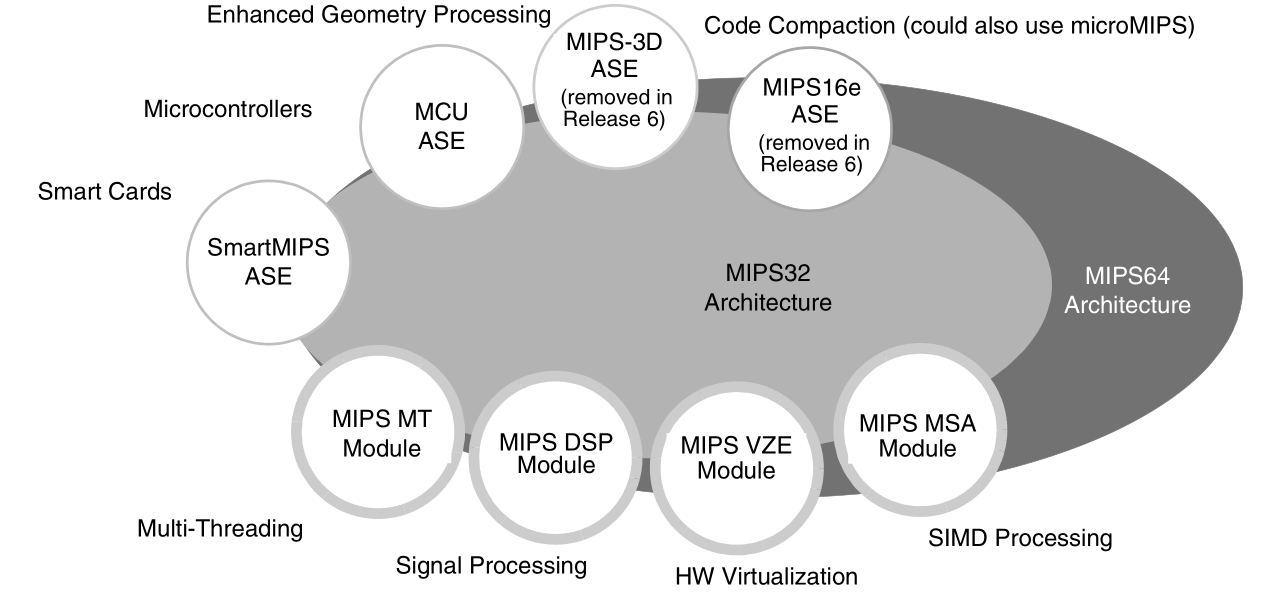
\includegraphics[width=\textwidth]{MIPS32_64_ASE_Modules}
			\end{frame}
			\begin{frame}
				\centering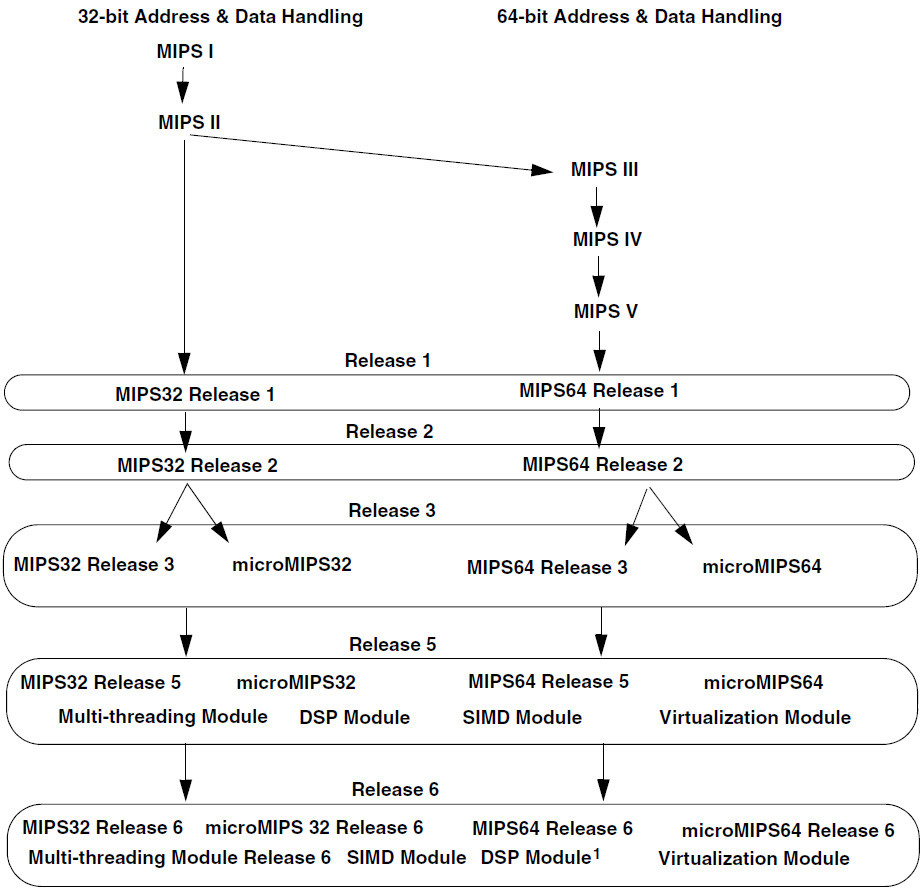
\includegraphics[width=0.55\textwidth]{MIPS_Architecture_Evolution}
				% 1985: MIPS I
				% 1999: MIPS32/64
				% 2012: R5
				% 2014: R6
			\end{frame}
			\begin{frame}
				\frametitle{MIPS32/64 Release 6}
				\centering\fbox{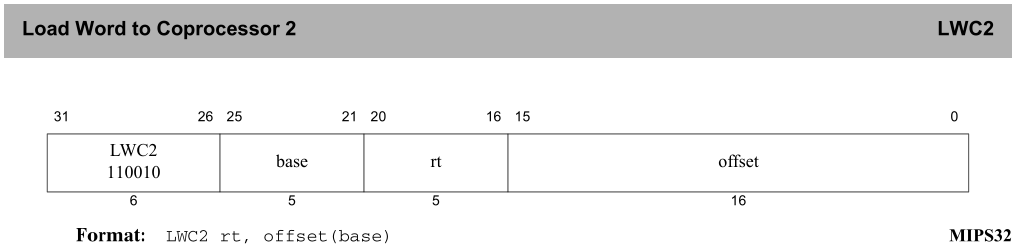
\includegraphics[width=0.9\textwidth]{MIPS_LWC2}}\\
				\centering\fbox{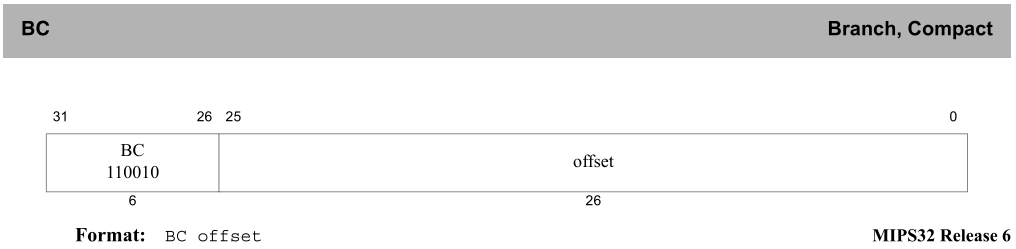
\includegraphics[width=0.9\textwidth]{MIPS_R6_BC}}
			\end{frame}
\end{document}
